\documentclass[a4paper,12pt]{article}
\usepackage[T1]{fontenc}
\usepackage[utf8]{inputenc}
\usepackage{polski}
\usepackage{color}
\usepackage{graphicx}
\usepackage{amsmath}
\usepackage{amssymb}
\usepackage{hyperref}
\usepackage{float}
\usepackage{listings}
\usepackage[backend=biber]{biblatex}

\addbibresource{bibliografia.bib}

\lstset{
  basicstyle=\ttfamily,
  columns=flexible,
  keepspaces=true,
  literate={ą}{{\k{a}}}1
           {ć}{{\'{c}}}1
           {ę}{{\k{e}}}1
           {ł}{{\l{}}}1
           {ń}{{\'{n}}}1
           {ó}{{\'{o}}}1
           {ś}{{\'{s}}}1
           {ź}{{\'{z}}}1
           {ż}{{\.{z}}}1
           {Ą}{{\k{A}}}1
           {Ć}{{\'{C}}}1
           {Ę}{{\k{E}}}1
           {Ł}{{\L{}}}1
           {Ń}{{\'{N}}}1
           {Ó}{{\'{O}}}1
           {Ś}{{\'{S}}}1
           {Ź}{{\'{Z}}}1
           {Ż}{{\.{Z}}}1
}

\title{Zadanie - wykład 2}
\author{Mikołaj Kubś, 272662}
\date{\today}

\begin{document}

\maketitle

\begin{figure}[H]
  \centering
  
\includegraphics[width=1\textwidth]{images/task.png}
  \caption{Opis zadania}
\end{figure}

\section{Kod kwerend}

\subsection{Kwerenda bez CTE}

\begin{lstlisting}[
  language=SQL,
  showspaces=false,
  basicstyle=\ttfamily,
  numbers=left,
  numberstyle=\tiny,
  commentstyle=\color{green},
  tabsize=2
  ]
SELECT TOP 20 
  p.Name AS "Nazwa produktu", 
  pc.Name AS "Nazwa kategorii", 
  SUM(sod.OrderQty) AS "Suma liczby sprzedanych"
FROM Sales.SalesOrderDetail sod
JOIN Production.Product p ON sod.ProductID = p.ProductID
JOIN Production.ProductSubcategory ps 
  ON p.ProductSubcategoryID = ps.ProductSubcategoryID
JOIN Production.ProductCategory pc 
  ON ps.ProductCategoryID = pc.ProductCategoryID
GROUP BY p.Name, pc.Name
ORDER BY "Suma liczby sprzedanych" DESC;
\end{lstlisting}

\subsection{Kwerenda z CTE}

\begin{lstlisting}[
  language=SQL,
  showspaces=false,
  basicstyle=\ttfamily,
  numbers=left,
  numberstyle=\tiny,
  commentstyle=\color{green},
  tabsize=2
  ]
WITH ProductSales AS (
    SELECT 
        p.Name AS ProductName, 
        SUM(sod.OrderQty) AS TotalQuantitySold,
		p.ProductSubcategoryID
    FROM Sales.SalesOrderDetail sod
    JOIN Production.Product p ON sod.ProductID = p.ProductID
    GROUP BY p.Name, p.ProductSubcategoryID
),
ProductCategories AS (
	SELECT
		p.ProductName,
		pc.Name AS CategoryName,
		p.TotalQuantitySold
	FROM ProductSales p		
    JOIN Production.ProductSubcategory ps 
      ON p.ProductSubcategoryID = ps.ProductSubcategoryID
    JOIN Production.ProductCategory pc 
      ON ps.ProductCategoryID = pc.ProductCategoryID
)
SELECT TOP 20
	ProductCategories.ProductName AS "Nazwa produktu",
	ProductCategories.CategoryName AS "Nazwa kategorii", 
	ProductCategories.TotalQuantitySold AS "Suma liczby sprzedanych"
FROM ProductCategories
ORDER BY TotalQuantitySold DESC;
\end{lstlisting}

\section{Wyniki}

\subsection{Porównanie wyników zwróconych przez obie kwerendy}

\begin{figure}[H]
  \centering
  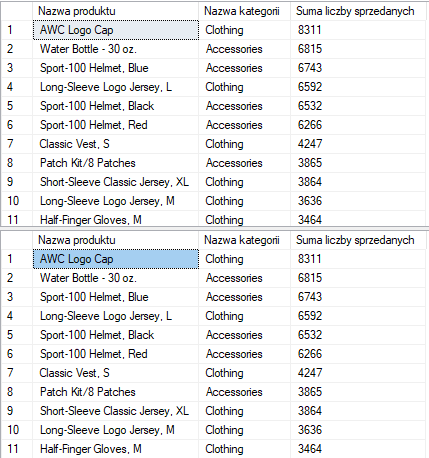
\includegraphics[width=1.0\textwidth]{images/results.png}
  \caption{Wyniki wykonania obu kwerend}
\end{figure}

Obie kwerendy zwracają identyczny zestaw wyników - 20 najlepiej sprzedających się produktów wraz z ich kategoriami. Użycie CTE nie wpływa na wynik końcowy, ale wpływa na sposób, w jaki dane są przetwarzane wewnętrznie.


\subsection{Porównanie różnic \textit{Execution Plan} dla obu kwerend}

\begin{figure}[H]
  \centering
  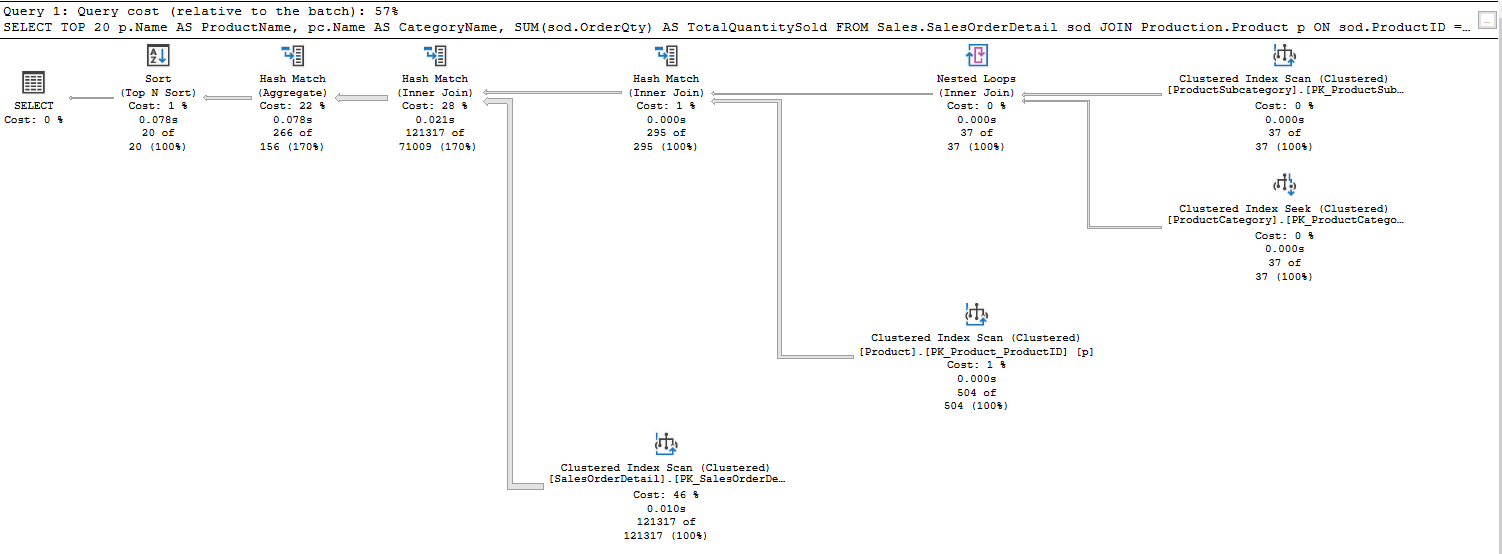
\includegraphics[width=1.0\textwidth]{images/query_1_plan.png}
  \caption{Execution Plan kwerendy bez CTE}
\end{figure}

\begin{figure}[H]
  \centering
  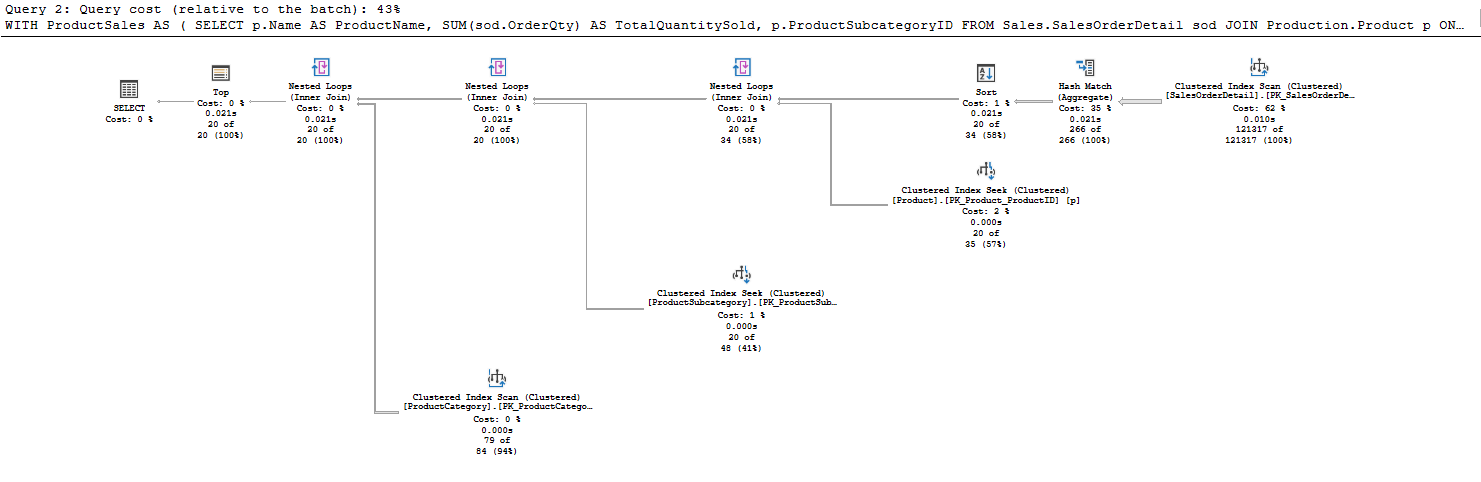
\includegraphics[width=1.0\textwidth]{images/query_2_plan.png}
  \caption{Execution Plan kwerendy z CTE}
\end{figure}

Przy dokładniejszej analizie widać sporo różnic pomiędzy kwerendami. Najważniejszą jest informacja, że "koszt" kwerendy z CTE wynosił 43\%, a kwerendy bez CTE 57\%. Tak więc "koszt" kwerendy z CTE wynosił około 75\% kosztu kwerendy bez CTE. Jest to całkiem znacząca różnica, a dla bardziej skomplikowanych kosztowo lub często wykonywanych kwerend każda optymalizacja jest istotna.

Dla kwerendy 1, sortowanie i limit zostało połączone w jeden krok, co zajęło nieznacznie więcej czasu niż osobne ich wykonanie w kwerendzie 2. Największą przewagą kwerendy 2 względem 1 jest to, że limit 20 był wzięty pod uwagę wcześniej, co pozwoliło na optymalizację szukania na przykład odpowiednich kategorii i subkategorii. Dane zostały zagregowane wcześniej, co sprawiło, że mniej wierszy trzeba było potem joinować.

\begin{figure}[H]
  \centering
  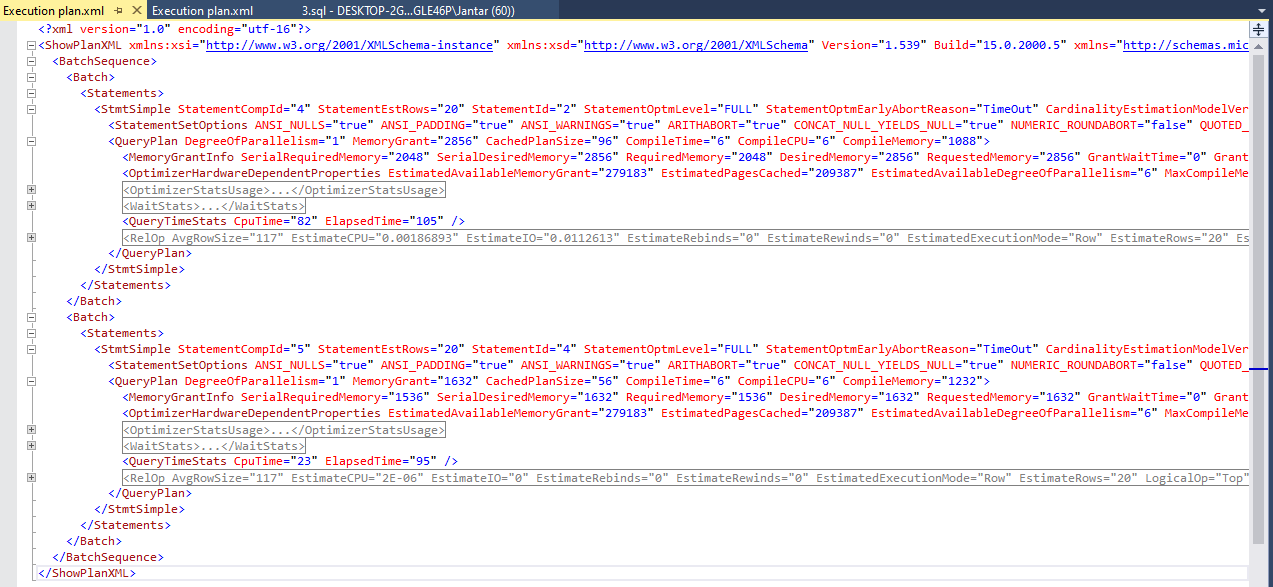
\includegraphics[width=1.0\textwidth]{images/memory_combined.png}
  \caption{Zrzut ekranu pliku XML zawierającego Execution Plan obu kwerend}
\end{figure}

"Koszt" kwerendy to nie tylko jej zużycie pamięci, a również CPU i operacje na dysku. Ale kwerenda 2 faktycznie zużywa nie tylko mniej zasobów niż kwerenda 1, ale też stricte mniej pamięci. Jak widać na powyższym obrazku, wszystkie statystyki odnośnie wymagań pamięci są mniejsze dla kwerendy z CTE. Kwerenda 2 dostała 1632 KB (GrantedMemory), a kwerenda 1 2856 KB. Oznacza to, że kwerenda bez CTE dostała 1,75 razy więcej pamięci niż zoptymalizowana kwerenda.


\section{Wnioski}

Analiza wykazała, że zastosowanie CTE pozwoliło na znaczące zmniejszenie zużycia pamięci (o około 43\%) oraz ogólnego kosztu zapytania. Dodatkowo podejście z CTE ułatwia dalszą i prostszą rozbudowę kwerendy oraz poprawia jej czytelność. Jednak dla bardzo prostych zapytań może nie być konieczne, a jego efektywność zależy od konkretnego przypadku i struktury danych.

\end{document}